\documentclass[10pt, twocolumn]{article}
\usepackage{graphicx} % Required for inserting images
\usepackage{float}
\usepackage{booktabs}
\usepackage[T1]{fontenc}
\usepackage[utf8]{inputenc}
\usepackage{lmodern}
\usepackage[english]{babel}
\usepackage[autostyle]{csquotes}
\usepackage{parskip}

\usepackage{comment}

\usepackage[backend=biber,style=authoryear]{biblatex}
\addbibresource{bibliography.bib}

\setlength{\parindent}{0px}


\title{Evaluating The Impact Of Water Harvesting For 4500+ Maasai in Communities In Monduli District, Arusha, Tanzania}
\author{Roshan Taneja, Yuvraj Taneja, Mbayani Tayai}
\date{April 2024}

\begin{document}

\maketitle

\begin{abstract}
In the Losimingori region in Tanzania, Maasai often walk to fetch water from nearby natural water bodies. In recent years, water harvesting solutions have been deployed in the region. The team's goal was to survey 35 families/individuals, representing approximately 500+ Maasai tribe members, to evaluate the impact of the 100k liter water harvesting unit's effectiveness that was deployed in 2022. The study found positive impacts on education, sanity, and quality of life. The direct impact of eliminating 7-8 hours of walking per day for 1500+ women and school children has resulted in investment in economic activity and agriculture and doubled school attendance. There is a wide range of water harvesting solutions that have the potential to affect the Maasai's daily lives and well-being significantly. Policymakers and practitioners should consider the potential benefits of such interventions when designing programs to address water scarcity and improve the livelihoods of communities in similar contexts.
\end{abstract}





















\section{Background}

Over two billion people worldwide cannot access clean water (\autocite{UNICEF2023}). This is a significant challenge for indigenous tribes and communities in Africa. A person in the US uses between 80 to 250 gallons of water per day (\autocite{EPA}). A Maasai uses less than ten gallons per day. Surprisingly, the annual rainfall in Tanzania is higher than the annual average in the United States (\autocite{Monduli}). Yet, the Maasai women spend up to nine hours daily fetching water. In addition, livestock, a major part of their livelihood, also need access to water, with over 30,000 Maasai distributed across a few 100 sq. miles. In Monduli, there is a huge dependence on access to water from the local Nanja Dam, specifically water access during extreme drought months (June to Nov).

\begin{figure} [H]
    \centering
    \includegraphics[width=1\linewidth]{photos/100k_unit.jpg}
    \caption{100k Litre Water Harvesting Unit [Completed June 2022]}
    \label{fig:100k_unit}
\end{figure}

% \begin{figure}
%     \centering
%     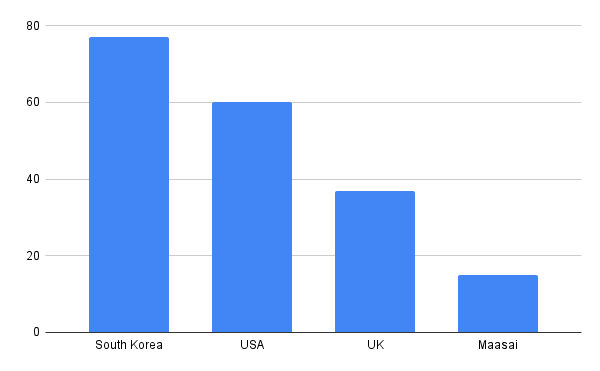
\includegraphics[width=1\linewidth]{photos/water_consumption.png}
%     \caption{Average water consumption per capita per day across multiple countries and the Maasai}
%     \label{fig:water_consumption}
% \end{figure}

Maji Wells is a non-for-profit organization based in the US focused on supporting the Maasai community in water, health, and education. "Maji" means water in Swahili. Maji Wells was founded by Mbayani Tayai, a local Maasai community member. The 100k liter water harvesting unit was deployed with the help of Maji Wells. The funds were raised by many supporting contributors, including the two authors of this paper. Funds were raised through many channels, including online social media platforms, phone calls, and email outreach. Roshan Taneja and Yuvraj Taneja fundraised \$20k in 2021 to contribute to this initiative. Maji Wells used local contractors and Lions Club Arusha's support to plan and install the 100k liter water harvesting unit for the Maasai community in Losimingori (Fig~\ref{fig:100k_unit}). A group of 5 US high school students led by Roshan Taneja and Maji Wells evaluated the impact on the community by surveying 35 families/individuals representing about 500+ Maasai tribe members. The unit was installed in June 2022 and returned; the data was collected in December 2022. The ultimate goal of the research was to understand the impact of the water harvesting unit on the finance, education, and culture of the Maasai. The findings of this study shed light on the effectiveness of the water harvesting unit in addressing the water needs of the Maasai people. It also emphasizes its broader impact on the community of the approximately 4500 people who use it.

\subsection{Literature Review}

\textbf{Rainwater Harvesting}

When considering the method of water distribution, two methods seemed most obvious. The two possible options are water wells or rainwater harvesting. Due to the over-drafting of groundwater, the area surrounding Arusha city has incredibly low or nonexistent water tables (\autocite{Ongor2007}). These shortcomings, In addition to Tanzania's high rainfall (Tab~\ref{tab:water_consumption}), rainwater harvesting is the most economically viable (\autocite{TZ_Water_Harvesting}) and sustainable.

\begin{table} [H]
    \begin{tabular}{@{}llll@{}}
    \toprule
    Country & \multicolumn{1}{l}{Gal} & Source &  \\ \midrule
    USA & 80 & (\autocite{USA_Water}) &  \\
    SK & 77 & (\autocite{SK_Water}) &  \\
    UK & 37 & (\autocite{UK_Water}) &  \\
    TZ & 16& Survey Data & \\ \bottomrule
    \end{tabular}
    \caption{Average water consumption per day per capita across multiple countries and the Maasai}
    \label{tab:water_consumption}
\end{table}

Rainwater harvesting is a method of collecting and storing rainwater for future use, and it is gaining traction as a sustainable water management system globally. It provides a decentralized, low-cost solution to water scarcity, specifically in areas with absent or unreliable conventional water supply systems. Rainwater harvesting is an easily affordable way to access clean water without filtration or other means of cleaning the water. Developing and developed nations have raised interest in rainwater harvesting technologies in the past few years. Due to the unpredictable nature of natural disasters and weather patterns, rainwater harvesting units have proven to be a useful way to alleviate the water strain in these areas. The method is particularly advantageous in regions with variable rainfall patterns, as it can buffer against periods of extreme drought. A house that captures 300ml of rainfall on 60 square meters of the roof could provide up to 50 Liters of water a day (\autocite{amos2018economic}).

(\autocite{kim2016community})

\textbf{Economic and Social Impacts}

Regularly available clean water has profound impacts on both economic and social life. In Ghana, reducing water fetching times has been linked to increased school attendance among girls, who no longer have to miss school to collect water (\autocite{Nauges2017}). Similarly, in Cambodia, providing safe drinking water through RWH systems has reduced absenteeism among schoolchildren during the dry season (\autocite{Cambodia_Water_Education}).

\textbf{Environmental and Technical Considerations}

Environmentally, RWH contributes to groundwater recharge, reduces surface runoff, and mitigates the risk of floods. It is also an adaptive strategy to climate change, offering resilience against weather extremes. Technically, the success of RWH systems depends on factors such as the design and capacity of the storage units, the quality of collected water, and the maintenance practices in place (\autocite{TZ_Water_Harvesting}).

\subsection{Procedure}

To ensure the most uniform dataset, demographic information was collected from those interviewed: 46\% were women, 23.3\% were older males, 23.3\% were "Moran" (Maasai young boys who are the tribe’s warriors between 15 and 25), and 7-8\% consisted of children(Blue) (Fig~\ref{fig:demographics}). Notably, a significant proportion of the interviewees (approximately 80\%) were interviewed at or near the water harvesting unit. To mitigate potential bias from interviewing respondents near the water harvesting unit, efforts were made to balance perspectives by interviewing individuals far from the unit. However, logistical constraints limited the ability to achieve a fully representative sample. Much of the Maasai community is inaccessible by road; therefore, interviewing outside of the Water harvesting units takes hours of walking several miles to each home. Due to limited time and resources, interviewing at the water harvesting unit provided many community members who used the units.

\begin{figure} [H]
    \centering
    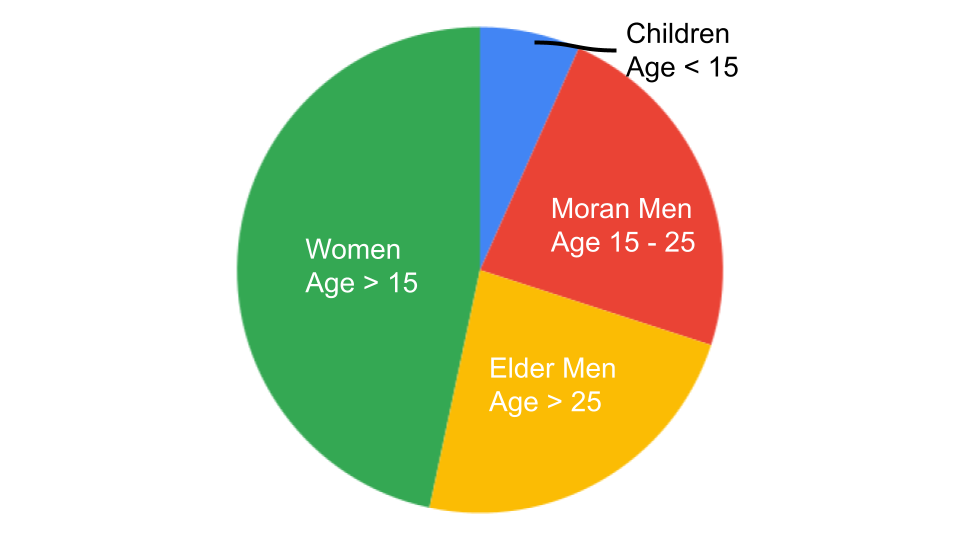
\includegraphics[width=1\linewidth]{photos/demographic_split.png}
    \caption{Demographics of Interviewees}
    \label{fig:demographics}
\end{figure}

We collected a selection of both qualitative and quantitative statistics. The qualitative data included open-ended responses about how the water unit affected daily life, perceptions of water quality, and changes in community dynamics. Respondents were asked to describe their activities with the extra time saved, the uses of water at home, and any perceived improvements in their quality of life. This narrative data provided rich insights into the personal and social impacts of the water units.

Quantitative data encompassed measures such as the amount of time saved by not walking to distant water sources, the frequency of water collection from the unit, and the volume of water collected. These metrics were crucial for assessing the practical benefits of the water units in terms of efficiency and usage patterns. Additionally, data on the distance from the water unit to respondents' homes, the duration for which collected water lasts, and the specific uses of the water at home were gathered to understand the logistical and functional aspects of water usage.

Unfortunately, the team did not collect a baseline comparison before implementing the water harvesting unit. The statistics on "Time Saved" and "current time" walking for water accurately estimate the initial time spent walking for water.

\subsection{Potential Biases}

There are several potential biases to be mindful of in this study:

\begin{itemize}
    \item \textbf{Location Bias:} Since most interviews were conducted near the water harvesting unit, there is a potential bias toward responses from those who regularly use and benefit from the unit. This could skew results toward more positive feedback about the water unit's impact.
    \item \textbf{Selection Bias:} The convenience sampling method used due to logistical constraints may not accurately represent the broader Maasai community. Those interviewed at the water unit might have different experiences and opinions compared to those living farther away who were less accessible.
    \item \textbf{Response Bias:} Respondents might provide socially desirable answers, especially if they perceive that positive feedback could lead to more resources or support from the researchers.
    \item \textbf{Interviewer Bias:} The presence and behavior of the interviewers could influence respondents' answers. Efforts to minimize this bias included training interviewers to remain neutral and consistent in their questioning.
\end{itemize}

















\section{Results}

We understood from preexisting studies that the Maasai walked nearly 60km daily for water collection (\autocite{choi2014salient}). Given the metrics for "Time Saved" and "Current time spent" walking for water, the estimated time spent walking for water is nearly 9 hours a day on average.

One of the key findings of this study is that 96\% of those interviewed reported using the water harvesting unit as their primary water source during the drought season. Maasai community members collect water between 3 am and 10 pm (\autocite{Google}). During the drought season, the water harvesting unit supports 4000+ community members. This underscores the importance of this unit in the daily lives of the Maasai people, particularly in areas where access to clean water is limited during the drought seasons. The use of the water harvesting unit as the primary source of water was consistent across different demographic groups, suggesting that the water harvesting unit is an effective and widely accepted solution for addressing the water needs of the Maasai people.

We found that 67.8\% of those interviewed continued using the water harvesting unit during the rainy season, indicating that the unit is helpful beyond just the dry season. Additionally, 82\% of those interviewed reported that they no longer had to walk long distances to fetch water from other sources, saving them valuable time. The median time saved daily was approximately 7 hours (Fig~\ref{fig:time_saved}). When asked what this extra time helps them do, some reported preparing jewelry to sell, while others harvested crops or cared for young boys and girls. Cleaning clothes and fencing were also mentioned as daily activities (Fig~\ref{fig:reallocation}).

\begin{figure}
    \centering
    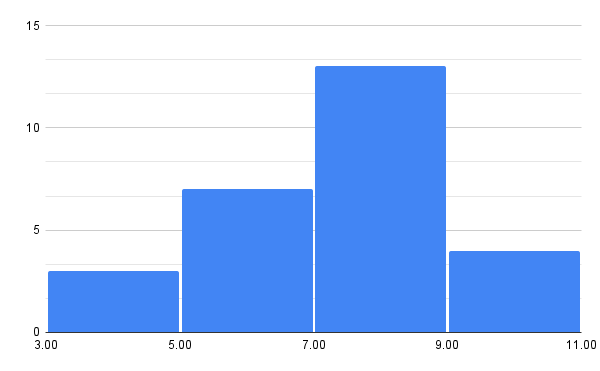
\includegraphics[width=1\linewidth]{photos/time_saved.png}
    \caption{Impact on time saved walking for water after construction.}
    \label{fig:time_saved}
\end{figure}

Our team also investigated the impact of the water harvesting unit on education. Three teachers [who taught in the local school about 1 mile from the Water Harvesting unit] reported that students came to school more cleanly and observed kids coming to school more often. Other research has also linked a positive impact on school attendance with access to water. (\autocite{Nauges2017}) Identified that "halving of water fetching times increases girls’ school attendance by about 7 percentage points on average, with stronger impacts in rural communities" while studying the relationship between hauling water and education in Ghana. (\autocite{Cambodia_Water_Education}) found "a strong association between providing free and safe drinking water and reduced absenteeism, although only in the dry season." In addition, the same teachers claimed to have seen an increase in the enrollment of new students. Although the exact reason is unclear, it's likely due to Maasai parents no longer requiring their children to haul water. This suggests that the availability of clean water positively impacts children's health and education outcomes in the Maasai community. Furthermore, 100\% of children who did not attend school before the installation of the water harvesting unit reported that their younger siblings were now being sent to school. This highlights the potential ripple effects of interventions like the water harvesting unit, which can positively impact the wider community. 

\begin{figure} [H]
    \centering
    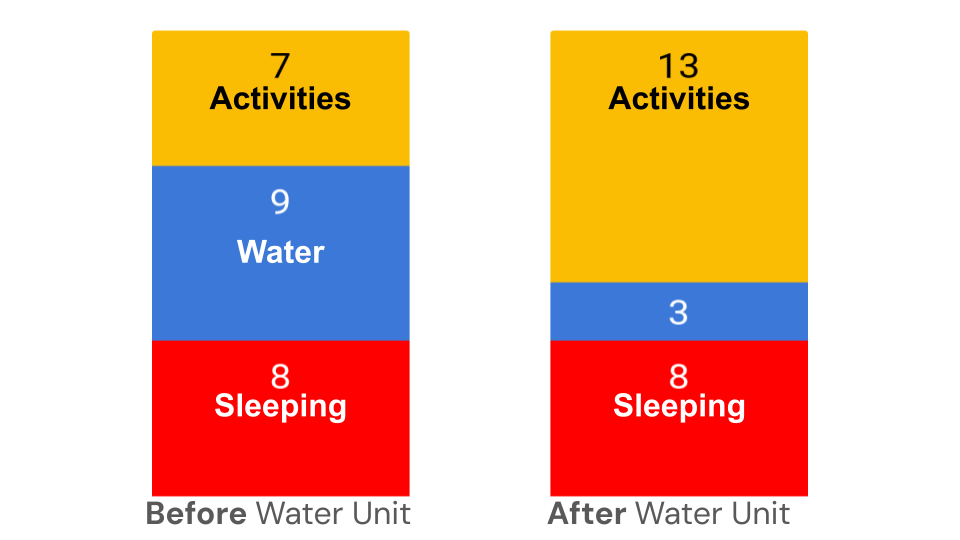
\includegraphics[width=1\linewidth]{photos/time_reallocation.png}
    \caption{Re-allocation of time saved}
    \label{fig:reallocation}
\end{figure}

These findings suggest that water harvesting units can have a significant impact on the daily lives and well-being of the Maasai people [Fig 6]. Policymakers and practitioners should consider the potential benefits of such interventions when designing programs to address water scarcity and improve the livelihoods of communities in similar contexts. A plan is being developed to introduce a universal water harvesting unit. The current water harvesting unit contains 100,000 liters when full. It would empty 3-4 days later, especially if all the members of the villagers depended on it. However, it is essential to note that the effectiveness of the water harvesting unit may depend on factors such as its proximity to households, the quality of the water collected, and the maintenance and upkeep of the unit over time. These factors should be considered when evaluating the impact of water harvesting units on the lives of the Maasai people.


















\section{Discussion}

Given the clear and robust positive evidence of the Water Harvesting Unit, three additional projects have been designed and executed between Nov 2022 and Feb 2023 (\autocite{Karimu}). These impacts will be measured in the next 6-12 months. Specifically:

\begin{enumerate}
    \item Another 40k litre Rainwater Harvest Tank in Losimingori (Fig~\ref{fig:40k_unit}).
    \item A Water filtration system (Fig~\ref{fig:filtration_unit}).
    \item Harvesting rainwater for irrigation (Fig~\ref{fig:irrigation_unit}).
\end{enumerate}

The water filtration system has been deployed in the village of Engirgiri, in Losimingori. The filtration unit cleans water from the local dam (man-made water ponds). This project was done with the villagers and the local water committee. The system uses simple technology, including the dam's water, two plastic tanks, an automatic solar water pump, Aluminium Sulphate, and Chlorine (Currently, at Maji Wells, a universal standard operating procedure (SOP) is being prepared, which will be a step-by-step, repeatable procedure. The SOP would organize the “must know” and “how to do” for the project – like a blueprint, guidelines, or operations manual.

For the Irrigation system, local farmers are empowered to create small ponds/ dams on their farms (pieces of land), harvest rainwater on the surface, and later use the harvested rainwater for irrigation during the dry season, plus introduce Poultry farming as a livestock alternative, which will not demand much water. This is a pilot project that the team wants to expand across all farmers. In addition, daily meteorological statistics for better data on local rain/dry days and seasons will be used to design the right size of water harvesting units and plan the locations for new water units.

\begin{figure}
    \centering
    \includegraphics[width=1\linewidth]{photos/40k_unit.JPG}
    \caption{Water Harvesting Unit of 40k Litres [completed Feb 2023]}
    \label{fig:40k_unit}
\end{figure}


\begin{figure}
    \centering
    \includegraphics[width=1\linewidth]{photos/water_filtration.JPG}
    \caption{Water Filtration [completed Feb 2023]}
    \label{fig:filtration_unit}
\end{figure}


\begin{figure}
    \centering
    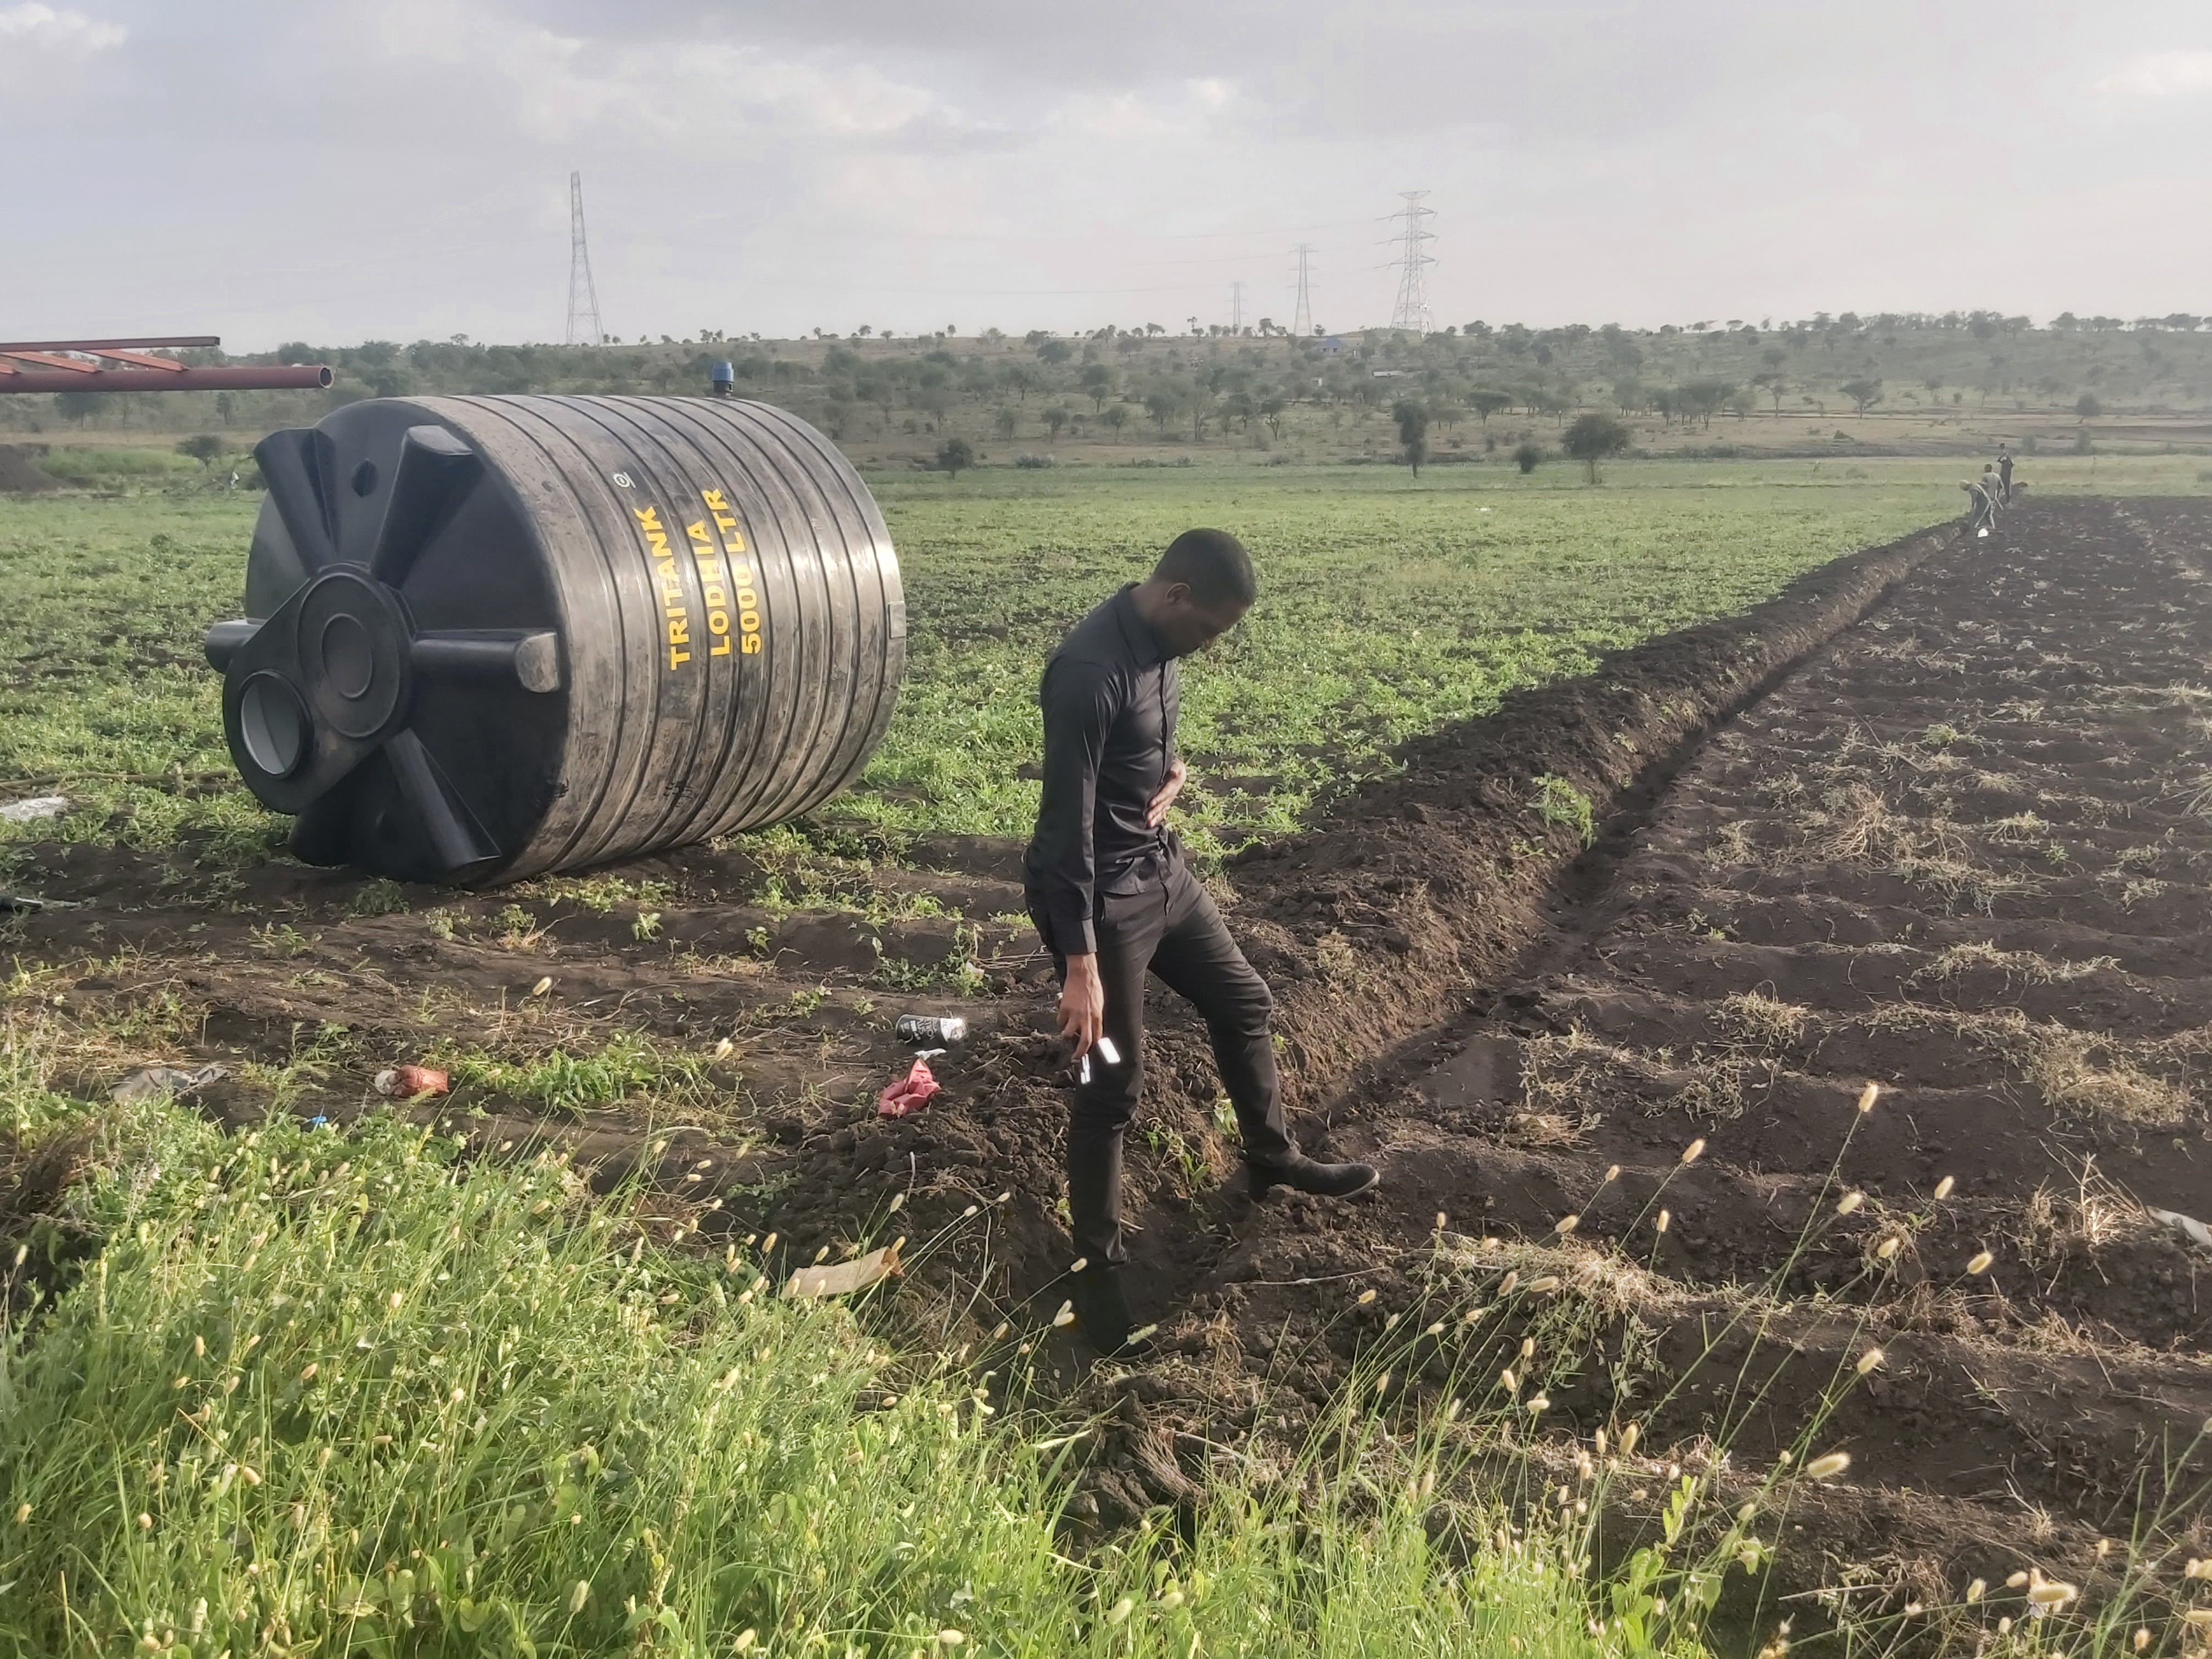
\includegraphics[width=1\linewidth]{photos/Irrigation_Unit.jpg}
    \caption{Water Harvesting Irrigation [completed Feb 2023]}
    \label{fig:irrigation_unit}
\end{figure}

Water councils have been established to ensure the sustainability and fair usage of the water harvesting units. The community's involvement in the maintenance of the units makes the whole initiative more scaleable and independent. These councils, composed of community members living closest to the water harvesting units, manage the units and oversee their maintenance. A small fee (approximately \$0.15 per liter) is charged when individuals draw more than 20 liters from the tank. The funds collected are used to maintain the units and, during the dry season, to hire water trucks from the city to refill smaller tanks that run low on water. The team also started measuring daily meteorological statistics for better data on local rain/dry days and seasons. This will help design the right size of water harvesting units and appropriately plan the locations for new water units.


















\section{Conclusion}

In conclusion, this study evaluated the positive impact of a 100k liter water harvesting unit installed by Maji Wells for the Maasai community in Losimingori, Tanzania. The research found that the water harvesting unit was widely effective and accepted by the community. Additionally, the availability of clean water positively impacted children's health and education outcomes, increasing school enrollment. The study underscores the importance of effective water management techniques to help communities like the Maasai cope with climate change and land degradation challenges. It is essential to acknowledge that many challenges still need to be addressed to ensure the sustainability of such solutions and interventions. By taking a holistic approach and involving the community in the planning and implementing such interventions, the benefits are long-lasting and contribute to the overall well-being and resilience of the community. In light of these findings, the program will continue to expand its impact via multiple projects: a subsidiary program that scales to 1000+ Maasai families [Bomas] impacting 15,000 population, additional filtration system for smaller dams, and placing more water harvesting units over the Monduli district, aimed at expanding the reach of these interventions and improving the livelihoods of 30,000 Maasai people in Monduli, Arusha region.















\section*{Acknowledgements}

\textbf{Research Team and contributors:} Adam Barycza (SHP), Arhaan Gupta-Rastogi (SHP), Joseph Shuaka, Kaay Lengima, Kanishk Pandey (DA), Mbayani Tayai, Roshan Taneja (SHP), Yuvraj Taneja (SHP)
\\ \newline
\textbf{Advisors:} Ayushi Jaiswal, Bala Bahl, Deepak Ramola, Nelson Mattos, Offir Inbar, Sharon Berkovich, Manish Chavda
\\ \newline
\textbf{Associated Organizations:} Maji Wells Foundation, Project FUEL, Karimu Foundation, Google Arts and Culture, Engineers Without Borders Tel Aviv, Lions Club: Arusha, Lions Club: Dar Es Salaam

\nocite{*}
\printbibliography

\section*{Contact}

Roshan Taneja:

Email: rytaneja [at] gmail [dot] com
\newline

Yuvraj Taneja:

Email: yuvrostan [at] gmail [dot] com
\newline

Mbayani Tayai:

Email: mbayanitayai [at] gmail [dot] com

\end{document}
